\documentclass{extbook}[14pt]
\usepackage{multicol, enumerate, enumitem, hyperref, color, soul, setspace, parskip, fancyhdr, amssymb, amsthm, amsmath, latexsym, units, mathtools}
\everymath{\displaystyle}
\usepackage[headsep=0.5cm,headheight=0cm, left=1 in,right= 1 in,top= 1 in,bottom= 1 in]{geometry}
\usepackage{dashrule}  % Package to use the command below to create lines between items
\newcommand{\litem}[1]{\item #1

\rule{\textwidth}{0.4pt}}
\pagestyle{fancy}
\lhead{}
\chead{Answer Key for Progress Quiz 6 Version B}
\rhead{}
\lfoot{9689-6866}
\cfoot{}
\rfoot{Spring 2021}
\begin{document}
\textbf{This key should allow you to understand why you choose the option you did (beyond just getting a question right or wrong). \href{https://xronos.clas.ufl.edu/mac1105spring2020/courseDescriptionAndMisc/Exams/LearningFromResults}{More instructions on how to use this key can be found here}.}

\textbf{If you have a suggestion to make the keys better, \href{https://forms.gle/CZkbZmPbC9XALEE88}{please fill out the short survey here}.}

\textit{Note: This key is auto-generated and may contain issues and/or errors. The keys are reviewed after each exam to ensure grading is done accurately. If there are issues (like duplicate options), they are noted in the offline gradebook. The keys are a work-in-progress to give students as many resources to improve as possible.}

\rule{\textwidth}{0.4pt}

\begin{enumerate}\litem{
Solve the rational equation below. Then, choose the interval(s) that the solution(s) belongs to.
\[ \frac{7x}{-2x -6} + \frac{-2x^{2}}{4x^{2} +26 x + 42} = \frac{7}{-2x -7} \]The solution is \( \text{There are two solutions: } x = 0.861 \text{ and } x = -3.049 \), which is option B.\begin{enumerate}[label=\Alph*.]
\item \( \text{All solutions lead to invalid or complex values in the equation.} \)


\item \( x_1 \in [-0.96, 2.07] \text{ and } x_2 \in [-3.12,-3.03] \)

* $x = 0.861 \text{ and } x = -3.049$, which is the correct option.
\item \( x \in [-3.17,-2.84] \)


\item \( x_1 \in [-0.96, 2.07] \text{ and } x_2 \in [-3.02,-2.99] \)


\item \( x \in [-4.26,-3.23] \)


\end{enumerate}

\textbf{General Comment:} Distractors are different based on the number of solutions. Remember that after solving, we need to make sure our solution does not make the original equation divide by zero!
}
\litem{
Determine the domain of the function below.
\[ f(x) = \frac{4}{15x^{2} -42 x + 24} \]The solution is \( \text{All Real numbers except } x = 0.800 \text{ and } x = 2.000. \), which is option D.\begin{enumerate}[label=\Alph*.]
\item \( \text{All Real numbers except } x = a, \text{ where } a \in [0.4, 1] \)

All Real numbers except $x = 0.800$, which corresponds to removing only 1 value from the denominator.
\item \( \text{All Real numbers.} \)

This corresponds to thinking the denominator has complex roots or that rational functions have a domain of all Real numbers.
\item \( \text{All Real numbers except } x = a \text{ and } x = b, \text{ where } a \in [17.7, 19.4] \text{ and } b \in [19.7, 20.7] \)

All Real numbers except $x = 18.000$ and $x = 20.000$, which corresponds to not factoring the denominator correctly.
\item \( \text{All Real numbers except } x = a \text{ and } x = b, \text{ where } a \in [0.4, 1] \text{ and } b \in [1.6, 2.5] \)

All Real numbers except $x = 0.800$ and $x = 2.000$, which is the correct option.
\item \( \text{All Real numbers except } x = a, \text{ where } a \in [17.7, 19.4] \)

All Real numbers except $x = 18.000$, which corresponds to removing a distractor value from the denominator.
\end{enumerate}

\textbf{General Comment:} Recall that dividing by zero is not a real number. Therefore the domain is all real numbers \textbf{except} those that make the denominator 0.
}
\litem{
Choose the graph of the equation below.
\[ f(x) = \frac{-1}{x - 2} - 2 \]The solution is the graph below, which is option B.
\begin{center}
    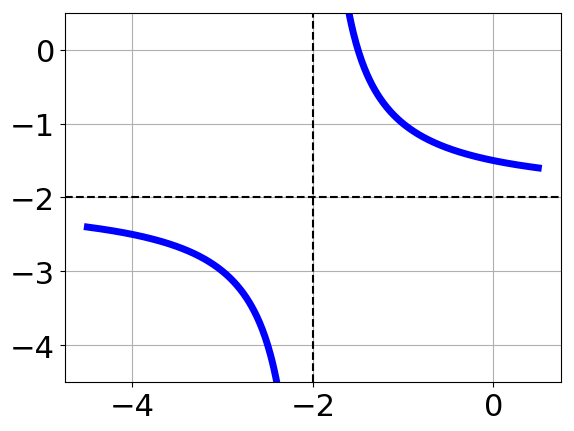
\includegraphics[width=0.3\textwidth]{../Figures/rationalEquationToGraphBB.png}
\end{center}\begin{enumerate}[label=\Alph*.]
\begin{multicols}{2}
\item 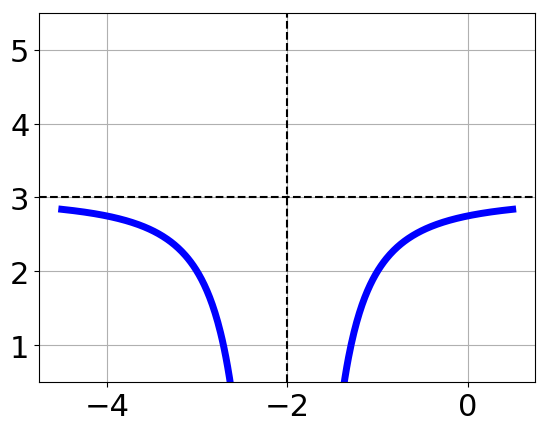
\includegraphics[width = 0.3\textwidth]{../Figures/rationalEquationToGraphAB.png}
\item 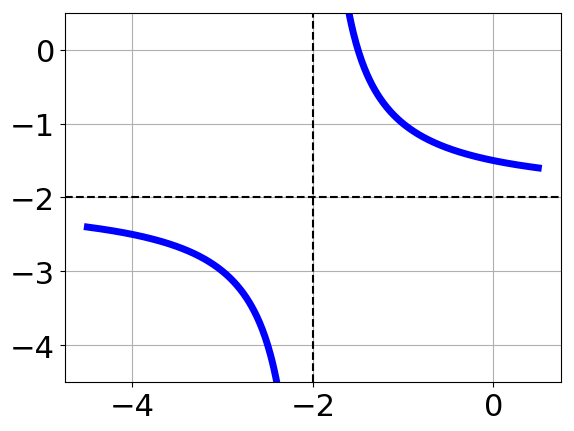
\includegraphics[width = 0.3\textwidth]{../Figures/rationalEquationToGraphBB.png}
\item 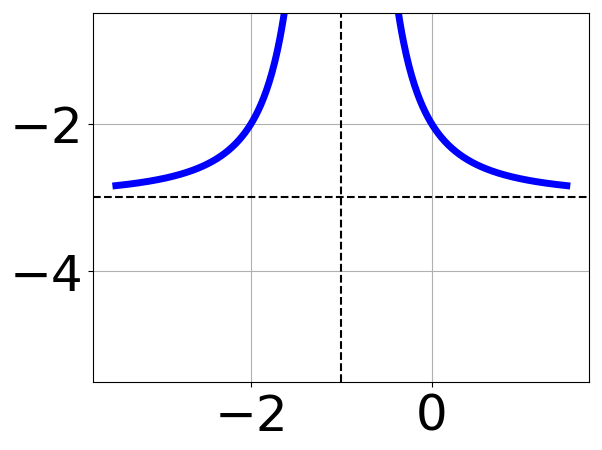
\includegraphics[width = 0.3\textwidth]{../Figures/rationalEquationToGraphCB.png}
\item 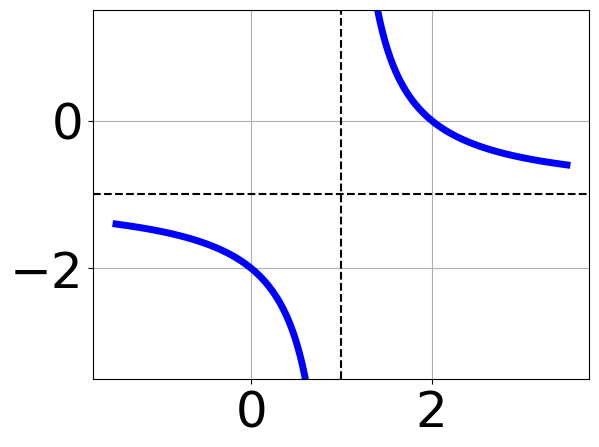
\includegraphics[width = 0.3\textwidth]{../Figures/rationalEquationToGraphDB.png}
\end{multicols}\item None of the above.\end{enumerate}
\textbf{General Comment:} Remember that the general form of a basic rational equation is $ f(x) = \frac{a}{(x-h)^n} + k$, where $a$ is the leading coefficient (and in this case, we assume is either $1$ or $-1$), $n$ is the degree (in this case, either $1$ or $2$), and $(h, k)$ is the intersection of the asymptotes.
}
\litem{
Choose the graph of the equation below.
\[ f(x) = \frac{1}{x - 1} - 3 \]The solution is the graph below, which is option E.
\begin{center}
    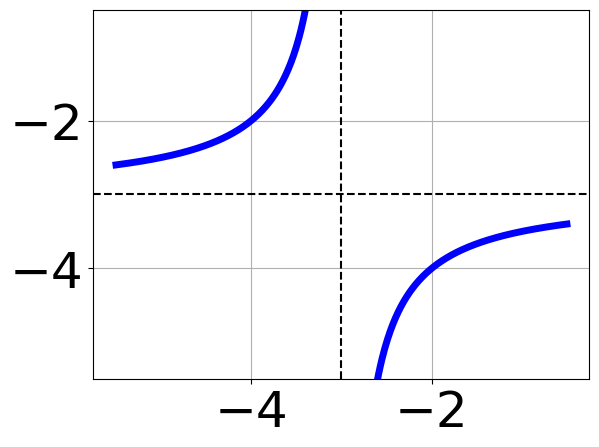
\includegraphics[width=0.3\textwidth]{../Figures/rationalEquationToGraphCopyEB.png}
\end{center}\begin{enumerate}[label=\Alph*.]
\begin{multicols}{2}
\item 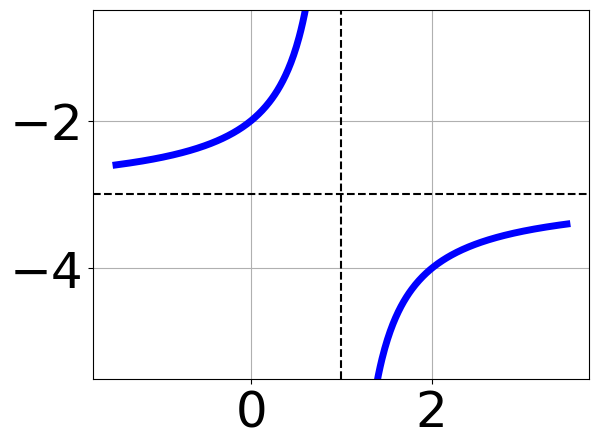
\includegraphics[width = 0.3\textwidth]{../Figures/rationalEquationToGraphCopyAB.png}
\item 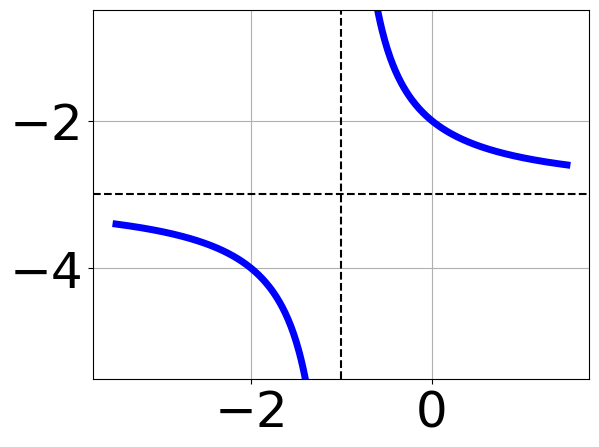
\includegraphics[width = 0.3\textwidth]{../Figures/rationalEquationToGraphCopyBB.png}
\item 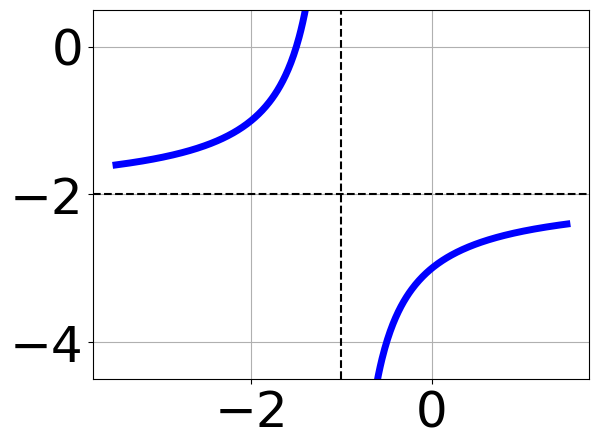
\includegraphics[width = 0.3\textwidth]{../Figures/rationalEquationToGraphCopyCB.png}
\item 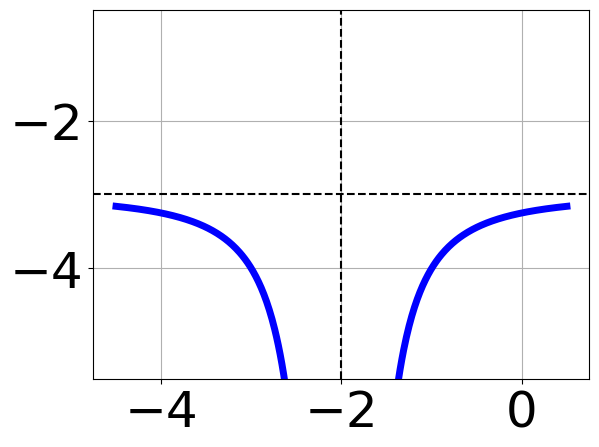
\includegraphics[width = 0.3\textwidth]{../Figures/rationalEquationToGraphCopyDB.png}
\end{multicols}\item None of the above.\end{enumerate}
\textbf{General Comment:} Remember that the general form of a basic rational equation is $ f(x) = \frac{a}{(x-h)^n} + k$, where $a$ is the leading coefficient (and in this case, we assume is either $1$ or $-1$), $n$ is the degree (in this case, either $1$ or $2$), and $(h, k)$ is the intersection of the asymptotes.
}
\litem{
Choose the equation of the function graphed below.

\begin{center}
    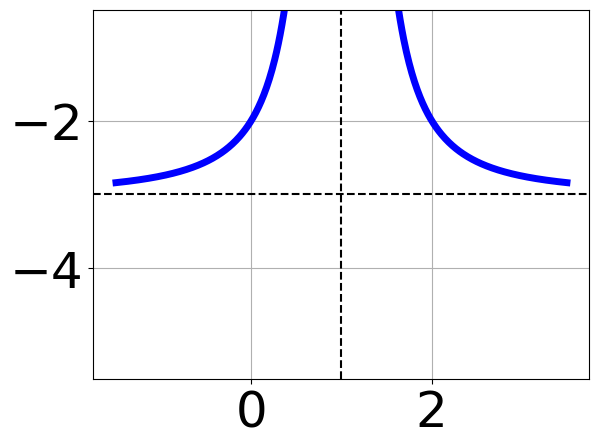
\includegraphics[width=0.5\textwidth]{../Figures/rationalGraphToEquationB.png}
\end{center}


The solution is \( f(x) = \frac{1}{x - 1} - 3 \), which is option C.\begin{enumerate}[label=\Alph*.]
\item \( f(x) = \frac{1}{(x - 1)^2} - 3 \)

Corresponds to thinking the graph was a shifted version of $\frac{1}{x^2}$.
\item \( f(x) = \frac{-1}{(x + 1)^2} - 3 \)

Corresponds to thinking the graph was a shifted version of $\frac{1}{x^2}$, using the general form $f(x) = \frac{a}{x+h}+k$, and the opposite leading coefficient.
\item \( f(x) = \frac{1}{x - 1} - 3 \)

This is the correct option.
\item \( f(x) = \frac{-1}{x + 1} - 3 \)

Corresponds to using the general form $f(x) = \frac{a}{x+h}+k$ and the opposite leading coefficient.
\item \( \text{None of the above} \)

This corresponds to believing the vertex of the graph was not correct.
\end{enumerate}

\textbf{General Comment:} Remember that the general form of a basic rational equation is $ f(x) = \frac{a}{(x-h)^n} + k$, where $a$ is the leading coefficient (and in this case, we assume is either $1$ or $-1$), $n$ is the degree (in this case, either $1$ or $2$), and $(h, k)$ is the intersection of the asymptotes.
}
\litem{
Choose the equation of the function graphed below.

\begin{center}
    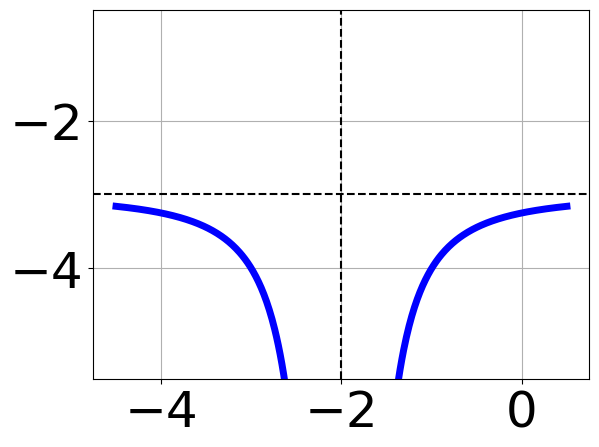
\includegraphics[width=0.5\textwidth]{../Figures/rationalGraphToEquationCopyB.png}
\end{center}


The solution is \( \text{None of the above as it should be } f(x) = \frac{-1}{(x + 2)^2} - 3 \), which is option E.\begin{enumerate}[label=\Alph*.]
\item \( f(x) = \frac{-1}{x - 2} - 6 \)

Corresponds to thinking the graph was a shifted version of $\frac{1}{x}$ AND not noticing the $y$-value was wrong.
\item \( f(x) = \frac{1}{x + 2} - 6 \)

Corresponds to thinking the graph was a shifted version of $\frac{1}{x}$, using the general form $f(x) = \frac{a}{(x-h)^2}+k$, the opposite leading coefficient, AND not noticing the $y$-value was wrong.
\item \( f(x) = \frac{-1}{(x - 2)^2} - 6 \)

The $x$- and $y$-value of the equation does not match the graph.
\item \( f(x) = \frac{1}{(x + 2)^2} - 6 \)

Corresponds to using the general form $f(x) = \frac{a}{(x-h)^2}+k$, the opposite leading coefficient, AND not noticing the $y$-value was wrong.
\item \( \text{None of the above} \)

None of the equation options were the correct equation.
\end{enumerate}

\textbf{General Comment:} Remember that the general form of a basic rational equation is $ f(x) = \frac{a}{(x-h)^n} + k$, where $a$ is the leading coefficient (and in this case, we assume is either $1$ or $-1$), $n$ is the degree (in this case, either $1$ or $2$), and $(h, k)$ is the intersection of the asymptotes.
}
\litem{
Solve the rational equation below. Then, choose the interval(s) that the solution(s) belongs to.
\[ \frac{-5}{8x -7} + 6 = \frac{3}{-56x + 49} \]The solution is \( x = 0.970 \), which is option E.\begin{enumerate}[label=\Alph*.]
\item \( \text{All solutions lead to invalid or complex values in the equation.} \)

This corresponds to thinking $x = 0.970$ leads to dividing by zero in the original equation, which it does not.
\item \( x_1 \in [-0.78, 0.22] \text{ and } x_2 \in [0.84,1.04] \)

$x = -0.780 \text{ and } x = 0.970$, which corresponds to getting the correct solution and believing there should be a second solution to the equation.
\item \( x \in [-0.78,0.22] \)

$x = -0.780$, which corresponds to not distributing the factor $8x -7$ correctly when trying to eliminate the fraction.
\item \( x_1 \in [-0.03, 1.97] \text{ and } x_2 \in [0.98,1.14] \)

$x = 0.970 \text{ and } x = 1.042$, which corresponds to getting the correct solution and believing there should be a second solution to the equation.
\item \( x \in [-0.03,1.97] \)

* $x = 0.970$, which is the correct option.
\end{enumerate}

\textbf{General Comment:} Distractors are different based on the number of solutions. Remember that after solving, we need to make sure our solution does not make the original equation divide by zero!
}
\litem{
Solve the rational equation below. Then, choose the interval(s) that the solution(s) belongs to.
\[ \frac{3}{4x -5} + 7 = \frac{-9}{-16x + 20} \]The solution is \( x = 1.223 \), which is option C.\begin{enumerate}[label=\Alph*.]
\item \( \text{All solutions lead to invalid or complex values in the equation.} \)

This corresponds to thinking $x = 1.223$ leads to dividing by zero in the original equation, which it does not.
\item \( x_1 \in [0.48, 0.92] \text{ and } x_2 \in [0.22,2.22] \)

$x = 0.821 \text{ and } x = 1.223$, which corresponds to getting the correct solution and believing there should be a second solution to the equation.
\item \( x \in [1.22,2.22] \)

* $x = 1.223$, which is the correct option.
\item \( x_1 \in [-1.68, -0.96] \text{ and } x_2 \in [0.22,2.22] \)

$x = -1.277 \text{ and } x = 1.223$, which corresponds to getting the correct solution and believing there should be a second solution to the equation.
\item \( x \in [-1.68,-0.96] \)

$x = -1.277$, which corresponds to not distributing the factor $4x -5$ correctly when trying to eliminate the fraction.
\end{enumerate}

\textbf{General Comment:} Distractors are different based on the number of solutions. Remember that after solving, we need to make sure our solution does not make the original equation divide by zero!
}
\litem{
Solve the rational equation below. Then, choose the interval(s) that the solution(s) belongs to.
\[ \frac{-2x}{-4x + 2} + \frac{-4x^{2}}{16x^{2} +4 x -6} = \frac{-6}{-4x -3} \]The solution is \( \text{There are two solutions: } x = 0.814 \text{ and } x = 3.686 \), which is option A.\begin{enumerate}[label=\Alph*.]
\item \( x_1 \in [0.4, 1.3] \text{ and } x_2 \in [1.69,10.69] \)

* $x = 0.814 \text{ and } x = 3.686$, which is the correct option.
\item \( x \in [-1.98,-0.23] \)


\item \( x \in [2.74,5.68] \)


\item \( x_1 \in [0.4, 1.3] \text{ and } x_2 \in [0.5,2.5] \)


\item \( \text{All solutions lead to invalid or complex values in the equation.} \)


\end{enumerate}

\textbf{General Comment:} Distractors are different based on the number of solutions. Remember that after solving, we need to make sure our solution does not make the original equation divide by zero!
}
\litem{
Determine the domain of the function below.
\[ f(x) = \frac{5}{36x^{2} -60 x + 24} \]The solution is \( \text{All Real numbers except } x = 0.667 \text{ and } x = 1.000. \), which is option D.\begin{enumerate}[label=\Alph*.]
\item \( \text{All Real numbers except } x = a \text{ and } x = b, \text{ where } a \in [23.69, 24.49] \text{ and } b \in [35.81, 36.63] \)

All Real numbers except $x = 24.000$ and $x = 36.000$, which corresponds to not factoring the denominator correctly.
\item \( \text{All Real numbers.} \)

This corresponds to thinking the denominator has complex roots or that rational functions have a domain of all Real numbers.
\item \( \text{All Real numbers except } x = a, \text{ where } a \in [0.55, 0.88] \)

All Real numbers except $x = 0.667$, which corresponds to removing only 1 value from the denominator.
\item \( \text{All Real numbers except } x = a \text{ and } x = b, \text{ where } a \in [0.55, 0.88] \text{ and } b \in [0.96, 1.28] \)

All Real numbers except $x = 0.667$ and $x = 1.000$, which is the correct option.
\item \( \text{All Real numbers except } x = a, \text{ where } a \in [23.69, 24.49] \)

All Real numbers except $x = 24.000$, which corresponds to removing a distractor value from the denominator.
\end{enumerate}

\textbf{General Comment:} Recall that dividing by zero is not a real number. Therefore the domain is all real numbers \textbf{except} those that make the denominator 0.
}
\end{enumerate}

\end{document}